% Options for packages loaded elsewhere
\PassOptionsToPackage{unicode}{hyperref}
\PassOptionsToPackage{hyphens}{url}
%
\documentclass[
  ignorenonframetext,
]{beamer}
\usepackage{pgfpages}
\setbeamertemplate{caption}[numbered]
\setbeamertemplate{caption label separator}{: }
\setbeamercolor{caption name}{fg=normal text.fg}
\beamertemplatenavigationsymbolsempty
% Prevent slide breaks in the middle of a paragraph
\widowpenalties 1 10000
\raggedbottom
\setbeamertemplate{part page}{
  \centering
  \begin{beamercolorbox}[sep=16pt,center]{part title}
    \usebeamerfont{part title}\insertpart\par
  \end{beamercolorbox}
}
\setbeamertemplate{section page}{
  \centering
  \begin{beamercolorbox}[sep=12pt,center]{part title}
    \usebeamerfont{section title}\insertsection\par
  \end{beamercolorbox}
}
\setbeamertemplate{subsection page}{
  \centering
  \begin{beamercolorbox}[sep=8pt,center]{part title}
    \usebeamerfont{subsection title}\insertsubsection\par
  \end{beamercolorbox}
}
\AtBeginPart{
  \frame{\partpage}
}
\AtBeginSection{
  \ifbibliography
  \else
    \frame{\sectionpage}
  \fi
}
\AtBeginSubsection{
  \frame{\subsectionpage}
}
\usepackage{lmodern}
\usepackage{amssymb,amsmath}
\usepackage{ifxetex,ifluatex}
\ifnum 0\ifxetex 1\fi\ifluatex 1\fi=0 % if pdftex
  \usepackage[T1]{fontenc}
  \usepackage[utf8]{inputenc}
  \usepackage{textcomp} % provide euro and other symbols
\else % if luatex or xetex
  \usepackage{unicode-math}
  \defaultfontfeatures{Scale=MatchLowercase}
  \defaultfontfeatures[\rmfamily]{Ligatures=TeX,Scale=1}
\fi
\usetheme[]{AnnArbor}
\usecolortheme{dolphin}
\usefonttheme{structurebold}
% Use upquote if available, for straight quotes in verbatim environments
\IfFileExists{upquote.sty}{\usepackage{upquote}}{}
\IfFileExists{microtype.sty}{% use microtype if available
  \usepackage[]{microtype}
  \UseMicrotypeSet[protrusion]{basicmath} % disable protrusion for tt fonts
}{}
\makeatletter
\@ifundefined{KOMAClassName}{% if non-KOMA class
  \IfFileExists{parskip.sty}{%
    \usepackage{parskip}
  }{% else
    \setlength{\parindent}{0pt}
    \setlength{\parskip}{6pt plus 2pt minus 1pt}}
}{% if KOMA class
  \KOMAoptions{parskip=half}}
\makeatother
\usepackage{xcolor}
\IfFileExists{xurl.sty}{\usepackage{xurl}}{} % add URL line breaks if available
\IfFileExists{bookmark.sty}{\usepackage{bookmark}}{\usepackage{hyperref}}
\hypersetup{
  pdftitle={MBP Tech Talks - DNA Sequencing},
  hidelinks,
  pdfcreator={LaTeX via pandoc}}
\urlstyle{same} % disable monospaced font for URLs
\newif\ifbibliography
\usepackage{graphicx,grffile}
\makeatletter
\def\maxwidth{\ifdim\Gin@nat@width>\linewidth\linewidth\else\Gin@nat@width\fi}
\def\maxheight{\ifdim\Gin@nat@height>\textheight\textheight\else\Gin@nat@height\fi}
\makeatother
% Scale images if necessary, so that they will not overflow the page
% margins by default, and it is still possible to overwrite the defaults
% using explicit options in \includegraphics[width, height, ...]{}
\setkeys{Gin}{width=\maxwidth,height=\maxheight,keepaspectratio}
% Set default figure placement to htbp
\makeatletter
\def\fps@figure{htbp}
\makeatother
\setlength{\emergencystretch}{3em} % prevent overfull lines
\providecommand{\tightlist}{%
  \setlength{\itemsep}{0pt}\setlength{\parskip}{0pt}}
\setcounter{secnumdepth}{-\maxdimen} % remove section numbering

\title{MBP Tech Talks - DNA Sequencing}
\date{}

\begin{document}
\frame{\titlepage}

\begin{frame}

\end{frame}

\begin{frame}{MBP Tech Talks}
\protect\hypertarget{mbp-tech-talks}{}

\begin{block}{Fall 2019}

Fundamentals of Genome Sequencing and Applications

\end{block}

\end{frame}

\begin{frame}{Motivations}
\protect\hypertarget{motivations}{}

\begin{itemize}
\tightlist
\item
  Lots of research involves genome sequencing or and analysis
\item
  Few resources covering the fundamentals
\item
  Information is often scattered through blog posts, presentations
\item
  Multidisciplinary - difficult for a single person to discuss
  thoroughly
\end{itemize}

\end{frame}

\begin{frame}{Goals for the fall semester}
\protect\hypertarget{goals-for-the-fall-semester}{}

\begin{itemize}
\tightlist
\item
  Understand foundations of genome sequencing

  \begin{itemize}
  \tightlist
  \item
    How DNA is captured and read
  \item
    What makes good sequencing data
  \end{itemize}
\item
  Sequence alignment
\item
  Wet and dry sides of sequencing experiments
\item
  How to think about good experiment design when sequencing
\end{itemize}

\end{frame}

\begin{frame}{Outline}
\protect\hypertarget{outline}{}

\begin{itemize}
\tightlist
\item
  Fundamentals of genome sequencing

  \begin{itemize}
  \tightlist
  \item
    History of reading DNA
  \item
    Massively-parallel sequencing
  \item
    Standard file formats
  \item
    Sequence alignment
  \item
    Alignment metrics
  \end{itemize}
\item
  Applications

  \begin{itemize}
  \tightlist
  \item
    Mutation detection
  \item
    Chromatin accessibililty
  \item
    Histone modifications and protein binding
  \item
    Transcriptome sequencing
  \item
    Chromatin organization
  \item
    DNA methylation
  \end{itemize}
\item
  Extended topics
\end{itemize}

\begin{block}{Session structure}

\begin{itemize}
\tightlist
\item
  HSB 100, Friday 12:00 - 14:00
\item
  No food or drinks
\item
  Each session has 2 parts, break in the middle
\end{itemize}

\end{block}

\end{frame}

\begin{frame}{DNA molecules}
\protect\hypertarget{dna-molecules}{}

\begin{figure}
\centering
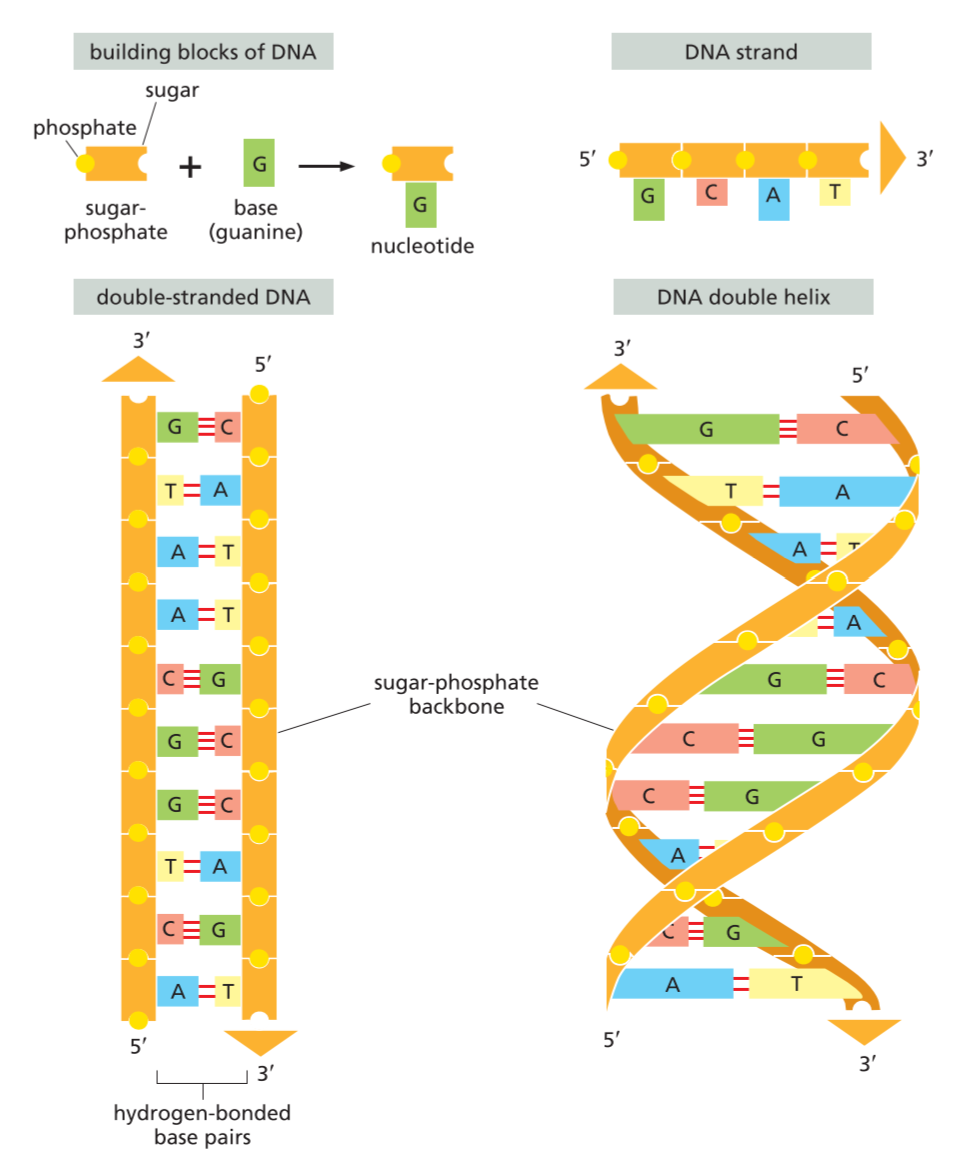
\includegraphics{dna-structure.png}
\caption{DNA structure}
\end{figure}

.footnote{[} {[}1{]} Alberts, Molecular biology of the cell, 6ed. pg.
176{]}

\begin{itemize}
\tightlist
\item
  DNA is double-stranded polymer

  \begin{itemize}
  \tightlist
  \item
    DNA contains 4 nucleotides: adenine (A), cytosine (C), guanine (G),
    thymine (T)
  \item
    DNA has a sugar-phosphate backbone
  \item
    Nucleotides come in complementary pairs: A-T, C-G
  \end{itemize}
\end{itemize}

\end{frame}

\begin{frame}{DNA molecules}
\protect\hypertarget{dna-molecules-1}{}

\begin{figure}
\centering
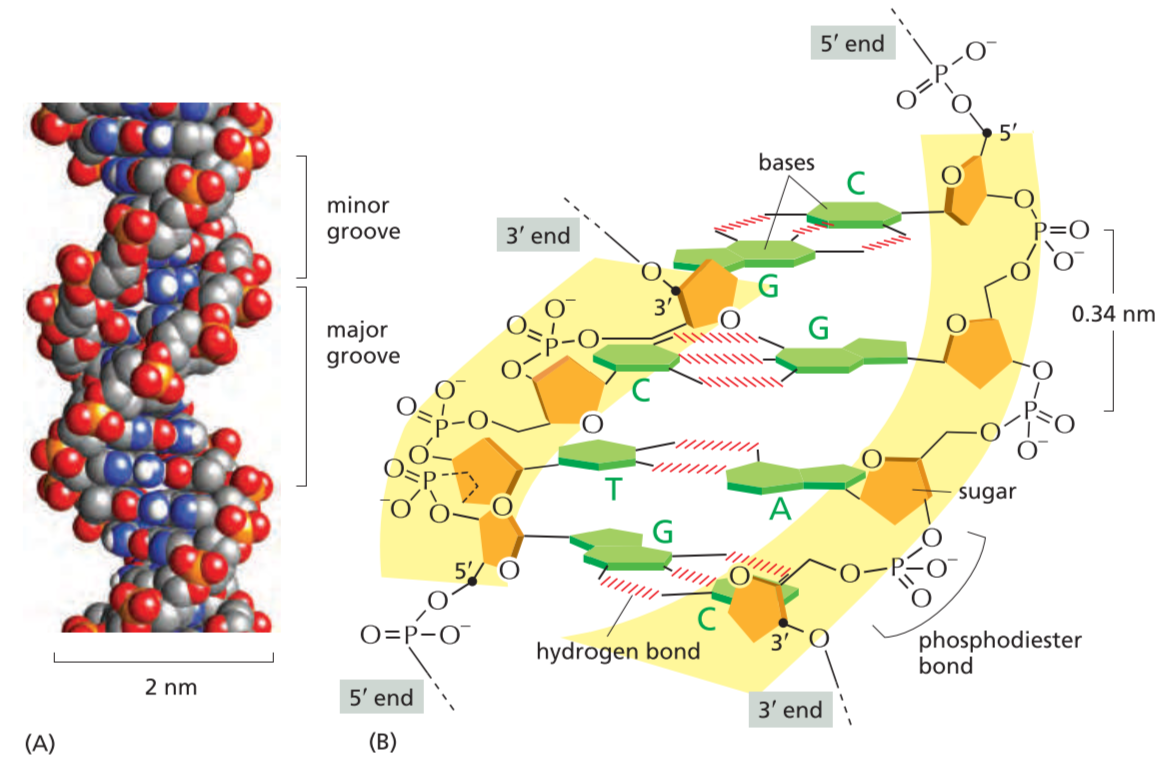
\includegraphics{dna-groove.png}
\caption{DNA structure}
\end{figure}

\begin{itemize}
\tightlist
\item
  DNA has a right-handed orientation

  \begin{itemize}
  \tightlist
  \item
    Strands are oriented in opposite directions
  \item
    We measure direction by counting 5' to 3'
  \end{itemize}
\end{itemize}

.footnote{[} {[}2{]} Alberts, Molecular biology of the cell, 6ed. pg.
177{]}

\end{frame}

\begin{frame}{DNA encodes information for organisms}
\protect\hypertarget{dna-encodes-information-for-organisms}{}

\begin{figure}
\centering
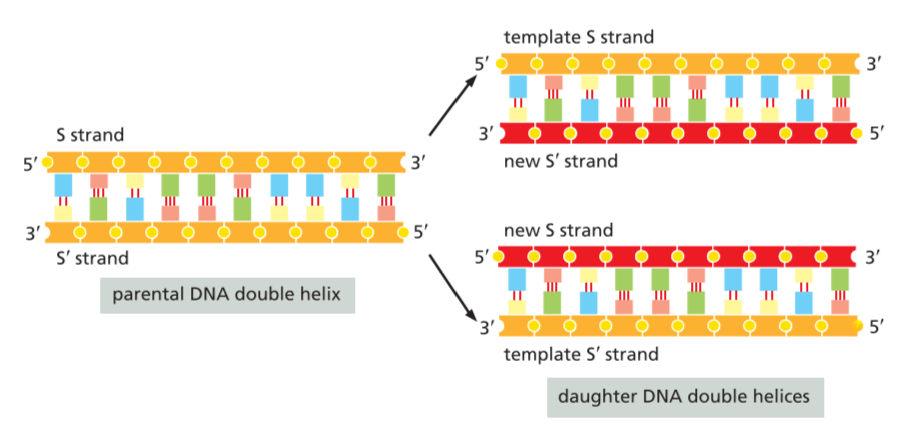
\includegraphics{dna-replication.png}
\caption{DNA replication}
\end{figure}

\begin{itemize}
\tightlist
\item
  Complementary strands allow for replication
\item
  Sequences themselves code for proteins inside cells
\item
  Genome: set of all DNA inside an organism/cell
\item
  DNA sequencing: the process of measuring the order of these
  nucleotides
\end{itemize}

.footnote{[} {[}3{]} Alberts, Molecular biology of the cell, 6ed. pg.
178{]}

\end{frame}

\begin{frame}{Early DNA sequencing - Sanger sequencing}
\protect\hypertarget{early-dna-sequencing---sanger-sequencing}{}

\end{frame}

\end{document}
